\section{GUI Programming}
\hspace*{0.5in} Python menyediakan berbagai pilihan untuk mengembangkan antarmuka pengguna grafis (GUIs). Yang paling tercantum dibawah ini : 

\begin{itemize}
\item Tkinter 

Antarmuka Python ke toolkit Tk GUI dikirimkan dengan Python.  
\item wxPython 

antarmuka Python open-source untuk wxWindows 
 
\item Jpython 

Port Python untuk java yang memberikan Python script akses tanpa batas ke perpustakaan kelas java pada mesin lokal 

\subsection{Tkinter Pemrograman} 
\hspace*{0.5in} Tkinter adalah perpustakaan GUI standar untuk Python. Python bila dikombinasikan dengan Tkinter menyediakan cara yang mudah dan cepat untuk membuat aplikasi GUI. Tkinter menyediakan antarmuka berorientasi ojek yang kuat untuk toolkit Tk GUI. 
 
\hspace*{0.5in} Membuat aplikasi GUI menggunakan Tkinter adalah tugas yang mudah. Yang diperlukan adalah melakukan langkah-langkah sebagai berikut : 
 
\item Mengimpor Tkinter modul 
\item Buat jendela utama aplikasi GUI 
\item Tambahkan satu atau lebih dari widget tersebut diatas ke aplikasi GUI 
\item Masukkan acara loop utama untuk mengambil tindakan terhadap setiap peristiwa dipicu oleh pengguna\end{itemize}
 
\vspace{12pt} 
Contoh : 
\begin{verbatim}
$  \#  $!/usr/bin/python} 
import Tkinter} 

top = Tkinter.Tk()} 

 $  \#  $ Code to add widgets will go here...} 

top.mainloop()} 
\end{verbatim}

\vspace{10pt}
\subsection{Tkinter Widget} 
\hspace*{0.5in} Tkinter menyediakan berbagai kontrol seperti tombol, label dan kotak teks yang digunakan dalam aplikasi GUI. Kontrol ini biasanya disebut widget.  
 
\hspace*{0.5in} Saat ini ada 15 jenis widget di Tkinter. Menyajikan widget serta penjelasan singkat pada tabel berikut ini : 
\vspace{100pt}


 %%%%%%%%%%%%  Table No:1 Here %%%%%%%%%%%%%%


\begin{table}[ht]
	\caption{Ukuran}
	\begin{tabular*}{\textwidth}{@{\extracolsep{\fill}}lcc}
		\hline
		Operator& Penjelasan \cr
		\hline
		Button&SMenampilkan tombol dalam aplikasi&\cr
		Canvas&Menggambar bentuk seperti garis, oval, poligon dan persegi panjang dalam aplikasi&\cr
		Checkbutton&Menampilkan sejumlah pilihan sebagai kotak centang. Pengguna dapat memilih beberapa pilihan pada suatu waktu&\cr
		Entry&Menampilka bidang garis teks tunggal untuk menerima nilai-nilai dari pengguna\cr
		Frame&Wadah untuk mengatur widget lainnya&\cr
		Label &Memberikan keterangan garis single untuk widget lainnya. Hal ini berisi gambar&\cr
		Listbox &Menyediakan daftar pilihan kepada pengguna&\cr
		Menubutton&Menampilkan menu dalam aplikasi&\cr
		Menu&Memberikan berbagai perintah untuk pengguna. Perintah-perintah ini terkandung di dalam MenuButton&\cr
		Message&Menampilkan bidang teks multiline untuk menerima nilai-nilai dari pengguna&\cr
		RadioButton&Menampilkan sejumah pilihan sebagai tombol radio. Pengguna dapat memilih hanya satu pilihan pada suatu waktu&\cr
		Scale&Menyediakan widget slide&\cr
		Scrollbar &Menambah kemampuan bergulir ke berbagai widget seperti kotak daftar&\cr
		Text&Menampilka teks dalam beberapa garis&\cr
		Toplevel&Menyediakan wajah jendela terpisah&\cr
		PanedWindow&Wadah yang mengandung sejumlah panel disusun horizontal atau vertikal&\cr
		LabelFrame&Wadah widget sederhana. Bertindak sebagai spacer atau wajah untuk layout jendela kompleks&\cr
		TkMessageBox&Menampilkan kotak pesan dalam aplikasi&\cr
		Spinbox &Memilih sejumlah tetap nilai-nilai&\cr
		\hline
	\end{tabular*}
	\begin{tablenotes}
	\end{tablenotes}
\end{table}


 %%%%%%%%%%%%  Table No:1 Ends Here %%%%%%%%%%%%%%


\vspace{12pt}
\hspace*{0.5in} Beberapa atribut sebagai ukuran, warna dan font ditentukan. Berikut adalah beberapa atribut standar : 
 
\begin{itemize}
\item Ukuran 
 
Berbagai panjang, lebar, dan dimensi lain dari widget digambarkan dalam banyak unit yang berbeda seperti : 
 
\item Jika menetapkan dimensi ke integer diasumsikan dalam piksel 
 
\item Menentukan unit dengan menentukan dimensi untuk string yang berisi sejumlah diikuti oleh :
\end{itemize}
\vspace{100pt}
 


 %%%%%%%%%%%%  Table No:2 Here %%%%%%%%%%%%%%


\begin{table}[ht]
	\caption{Ukuran}
	\begin{tabular*}{\textwidth}{@{\extracolsep{\fill}}lcc}
		\hline
		Karakter&  Penjelasan \cr
		\hline
		c&Sentimeter&\cr
		i&Inci&\cr
		m&Milimeter&\cr
		p&Poin printer\cr
		\hline
	\end{tabular*}
	\begin{tablenotes}
	\end{tablenotes}
\end{table}


 %%%%%%%%%%%%  Table No:2 Ends Here %%%%%%%%%%%%%%


\hspace*{0.5in} Tkinter mengungkapkan panjang sebagai integer jumlah piksel. Berikut ini adalah daftar pilihan panjang umum: 
 
\begin{itemize}
\item borderwidth 

Lebar batas yang memberikan tampilan tiga dimensi untuk widget 
\item highlightthickness 

Lebar puncak persegi panjang ketika widget memiliki fokus 
\item padX padY 

Ruang tambahan widget dari manajer tata letak luar minimum widget perlu menampilkan isinya di x dan y arah 
\item selectborderwidth 

Lebar perbatasan tiga dimensi disekitar dipilih item widget 
\item wraplength 

Panjang garis maksimum untuk widget yang melakukan kata membungkus 
\item height 

Tinggi diinginkan widget 
\item underline 

Indeks karakter untuk menggarisawahi dalam teks widget  
\item width 
 
\item Lebar diinginkan widget

\item Warna 
\end{itemize}
\vspace{12pt}
 
\hspace*{0.5in} Tkinter memiliki warna dengan string. Ada dua cara umum untuk menentukan warna di Tkiter, yaitu : 
 
\begin{itemize}
\item Menggunakan string menentukan proporsi merah, hijau dan biru didigit heksadesimal. Misalnya  $ " $ $  \#  $ffff $ " $ putih,  $ " $ $  \#  $000000 $ " $ hitam dan  $ " $ $  \#  $000fff000 $ " $ hijau. 
 
\item Menggunakan lokal standar nama warna . warna-warna  $ " $white $ " $, $ " $black $ " $,  $ " $green $ " $ dan  $ " $magenta $ " $ akan selalu tersedia.\end{itemize}
 
\vspace{12pt}
Pilihan warna umum : 
 
\begin{itemize}
\item activebackground 

Warna latar berlakang untuk widget ketika widget aktif 
\item activeforeground 

Warna depan untuk widget ketika widget aktif 
\item background 

Merepresentasikan sebagai \textit{bg} 
\item disableforeground 

Warna depan untuk widget ketika widget dinonaktifkan 
\item foreground 

Merepresentasikan fg 
\item highlightbackground 

Warna latar belakang dari daerah puncak ketika widget memiliki fokus 
\item hightlightcolor 

Warna depan dari wilayah puncak ketika widget memiliki fokus 
\item selectbackground 

Warna latar belakang untuk item yang dipilih dari widget 
\item selectforeground 

Warna depan untuk item yang dipilih dari widget 
\item Font 
 
Sebagai tupel yang elemen pertama adalah keluarga font diikuti dengan string yang berisi satu atau lebih gaya pengubah tebal,miring, garis bawah dan overstrike. 
\end{itemize}
 
\vspace{12pt}
\hspace*{0.5in} Dapat membuat  $ " $font object $ " $ dengan mengimpor modul tkFont dan menggunakan kelas konstruktor font nya : 
Import tkFont 
Font = tkFont.Font (option, ....) 
\vspace{12pt}
Berikut adalah daftar pilihan : 
 
\begin{itemize}
\item Family 

Font nama keluarga sebagai string 
\item Size 

Font tinggi sebagai integer dalam poin 
\item Weight 

Bold untuk teal, normal untuk berat badan secara teratur 
\item Slant 

Italic untuk miring, roman untuk unstlanted 
\item Underline 

1 untuk teks yang digarisbawahi, 0 untuk normal 
\item Overstrike 

1 untuk teks telak, 0 untuk normal 
Jika berjalan di bawah X window system, dapat menggunakan salah satu nama font X. Sebagai contoh, font bernama  $ " $-*lucidatypewriter-medium-r-*-*-*-140-*-*-* $ " $ adalah favorit fixed-width font penulis untuk digunakan pada layar. 
\item Jangkar  

Jangkar digunakan untuk mendefinisikan mana teks diposisikan relatif terhadap titik acuan. 
\end{itemize}
 
\vspace{12pt}
\hspace*{0.5in} Jika menggunakan tengah sebagai jangkar tek, tek akan ditengahkan horizontal dan vertikal disekitar titik referensi. 
Jangkar NW akan posisi teks sehingga titik referensi bertepatan dengan laut sudut kotak berisi teks 
Jangakr W akan pusat teks secara vertikal disekitar titik referensi dengan tepi kiri kotak teks yang melewati titik itu dan sebagainya. 
Jika membuat widget kecil didalam bingkai besar dan menggunakan jangkar = SE pilihan, widget akan ditempatkan disudut kanan bawah gambar. Jika menggunakan anchor = N sebaliknya widget akan dipusatkan disepanjang tepi atas. 

\hspace*{0.5in}Widget mengacu pada efek 3-D simulasi terbaru disekitar bagian luar widget. Berikut adalah daftar konstanta yang mungkin dapat digunakan untuk atribut: 
 
\begin{itemize}
\item Datar 
 
\item Dibesarkan 
 
\item Cekung 
 
\item Alur 
 
\item Punggung bukit
\end{itemize}
 
\vspace{12pt}
Contoh : 
\begin{verbatim}
From Tkinter import *} 

Import Tkinter} 

 top = Tkinter.Tk()} 
B1 = Tkinter.Button(top, text= $ " $FLAT $ " $, relief
=FLAT)} 
B2 = Tkinter.Button(top, text= $ " $RAISED $ " $, relief
=RAISED)} 
B3 =Tkinter.Button(top, text= $ " $SUNKEN $ " $, relief
=SUNKEN)} 
B4=Tkinter.Button(top, text= $ " $GROOVE $ " $, relief
=GROOVE)} 
B5=Tkinter.Button(top, text= $ " $RIDGE $ " $, relief
=RIDGE)} 

 B1.pack()} 
 B2.pack()} 
 B3.pack()} 
 B4.pack()} 
 B5.pack()} 
 top.mainloop()} 
 \end{verbatim}
 
Ada beberapa jenis bitmap yang tersedia, diantaranya:  
\begin{itemize}
\item Kesalahan 
 
\item Gray75 
 
\item Gray50 
 
\item Gray12 
 
\item Jam Pasir 
 
\item Info 
 
\item Questhead 
 
\item Perantanyaan  
 
\item Peringatan\end{itemize}
 
\vspace{12pt}
Contoh: 
\begin{verbatim}
 From Tkinter import *} 
 
 Import Tkinter} 

 Top = Tkinter.Tk()} 

 B1 = Tkinter.Button(top, text = $ " $error $ " $, relief
 =RAISED,  $    $ bitmap= $ " $error $ " $)} 
 B2 = Tkinter.Button(top, text = $ " $hourglass $ " $, relief
 =RAISED,  $    $ bitmap= $ " $hourglass $ " $)} 
 B3 = Tkinter.Button(top, text = $ " $info $ " $, relief
 =RAISED,  $    $ bitmap= $ " $info $ " $)} 
 B4 = Tkinter.Button(top, text = $ " $question $ " $, relief
 =RAISED,  $    $ bitmap= $ " $question $ " $)} 
 B5 = Tkinter.Button(top, text = $ " $warning $ " $, relief
 =RAISED,  $    $ bitmap= $ " $warning $ " $)} 

 B1.pack()} 
 B2.pack()} 
 B3.pack()} 
 B4.pack()} 
 B5.pack()} 
 top.mainloop()} 
\end{verbatim}

\vspace{12pt}
Berikut daftar menarik : 
 
\begin{itemize}
\item Panah 
 
\item Lingkaran 
 
\item Jam 
 
\item Menyebrang 
 
\item Dotbox 
 
\item Bertukar 
 
\item Fluer 
 
\item Jantung 
 
\item Manusia 
 
\item Tikus 
 
\item Bajak laut 
 
\item Tamah 
 
\item Antar jemput 
 
\item Perekat 
 
\item Laba-laba 
 
\item Kaleng semprot 
 
\item Bintang 
 
\item Target 
 
\item Tcross 
 
\item Melakukan perjalanan 
 
\item Menonton
\end{itemize}
 
\vspace{12pt}
Contoh : 
\begin{verbatim}
From Tkinter import *} 

Import Tkinter} 

Top = Tkinter.Tk()} 

B1 = Tkinter.Button(top, text = $ " $circle $ " $, relief
=RAISED,  $    $ bitmap= $ " $circle $ " $)} 
B2 = Tkinter.Button(top, text = $ " $plus $ " $, relief
=RAISED,  $    $ bitmap= $ " $plus $ " $)} 

B1.pack()} 
B2.pack()} 
font top.mainloop()} 
\end{verbatim}

\vspace{10pt}
\subsection{Manajemen Geometri} 
 
\hspace*{0.5in} Semua widget tkinter memiliki akses ke metode manajemen geometri tertentu, yang memiliki tujuan menggorganisir widget diseluruh wilayah widget induk. Tkinter mengekspos kelas manager geometri berikut : 
 
\begin{itemize}
\item Metode the \textit{pack()} 
 
Manajer geometri ini mengatur widget diblok sebelum menempatkan mereka di widget induk 
\item Metode the \textit{grid()} 
 
Manajer geometri ini mengatur widget dalam struktur tabel seperti di widget induk 
\item Metode~the  \textit{place()}\end{itemize}
  
Manajer geometri ini mengatur widget dengan menempatkan dalam posisi tertentu dalam widget induk 
\vspace{12pt}
 
\subsection{Manfaat Tkinter} 
\hspace*{0.5in} Tkinter sangat sederhana. Erikut manfaat Tkinter dibandingkan GUI toolkit : 
 
\begin{itemize}
\item Tkinter mudah diakses oleh siapa saja (Accessibilty)

Tkinter merupakan toolkit yang ringan dan satu-satunya solusi GUI yang paling sederhana untuk Python sampai saat ini. Cukup menuliskan beberapa baris kode Python untuk membuat aplikasi GUI sederhana dengan Tkinter. Untuk menambahkan komponen baru pada Tkinter, dapat membuatnya dalam kode Python atau menambahkan paket ekstensi seperti Pmw, Tix, atau ttk. 
\item Tkinter mudah digunakan di semua platform (Portability)

Sebuah program Python yang dibangun menggunakan Tkinter dapat berjalan dengan baik di semua platform sistem operasi seperti Microsoft Windows, Linux, dan Macintosh. Dan dari segi tampilan window, akan terlihat sama dengan standar platform yang digunakan. 
 
\item Tkinter selalu tersedia di Python (Availability)

Tkinter merupakan modul standar pada pustaka Python. Sebagian besar paket instalasi Python sudah langsung berisi Tkinter. Khusus untuk beberapa distro Linux, perlu menambahkan paket Tkinter secara terpisah. Pada Windows, bisa langsung menggunakan Tkinter sesaat setelah menginstal paket instalasi Python. 
 
\item Dokumentasi Tkinter (Documentation)

Python (plus Tkinter) ini bersifat open-source, maka banyak sekali komunitas-komunitas yng membahas Python dan Tkinter dan bisa belajar dan bertanya langsung dengan para ahli
\end{itemize}

\section{Contoh GUI Programming}
\hspace*{0.5in} Dalam contoh ini, menulis naskah yang membuka jendela yang memiliki dua kotak masuk diantaranya satu nama depan berlabel dan nama belakang lainnya. Jendela memiliki dua tombol yaitu Greeting yang menampilkan kotak pesan selamat datang ke pengguna dan Close yang menutup aplikasi

\begin{verbatim}
import tkinter
from tkinter import *

det DisplayMsgBox():

    tkinter.messagebox.showinfo("Your Name", "Welcome"+ 
    Entry.get()+ "" +Entry2.get())

mainwindow = Tk()
Label(mainwindow, text="Firstname").grid(row=0)
Label(mainwindow, text="Lastname").grid(row=0)

Entry1 = Entry(mainwindow)
Entry2 = Entry(mainwindow)

Entry1.grid(row=0, column=1)
Entry2.grid(row=1, column=1)
Entry1.focus()

Button(mainwindow, text='Greeting', command=DisplayMsgBox)
.grid(row=3, column=0)
Button(mainwindow, text='Close', command=DisplayMsgBox)
.grid(row=3, column=1)

mainloop()
\end{verbatim}

\vspace{12pt}
Ketik nama depan dan nama belakang, lalu tekan "Greeting", \ref{Contoh} Lihat Contoh dibawah ini :
\begin{figure}[ht]
	\centerline{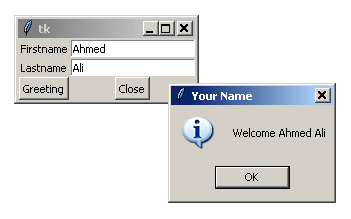
\includegraphics[width=0.70\textwidth]{figures/Contoh}}
	\caption{Contoh}
	\label{Contoh}
\end{figure}

\vspace{12pt}
Tekan "Close" akan menghentikan aplikasi 

*******

\vspace{12pt}
\hspace*{0.5in} Tkinter berisi sebagian besar kelas dan metode yang dibutuhkan untuk membuat aplikasi GUI yang bagus. Menggunakan kelas Tk untuk membuat master (jendela utama) dan instantiated objek untuk memasukkan berbagai kontrol pada jendela aplikasi.

